\documentclass[a0]{sciposter}
\usepackage{lipsum}
\usepackage{epsfig}
\usepackage{amsmath}
\usepackage{amssymb}
\usepackage{multicol}
\usepackage{graphicx,url}
\usepackage[spanish, brazil]{babel}   
\usepackage[utf8]{inputenc}
%\usepackage{fancybullets}
\newtheorem{Def}{Definition}

\newcommand{\groupname}{\textbf{Termodinámica de Soluciones}}
\newcommand{\grad}{$^\circ$C}

\title{Puesta en marcha y calibración de un	calorímetro\\ 2277 de ThermoMetric}
%Título do projeto

\author{Juan \textsc{Barbosa}\\dirigido por Edgar F. \textsc{Vargas}, Dr.Sc.}
%nome dos autores

\institute 
{Departamento de Qu\'imica\\
	Universidad de los Andes\\
	Cra 1 N$^\circ$ 18A - 12 Bogotá, Colombia}

\email{js.barbosa10@uniandes.edu.co}

%\rightlogo[1]{logo}
\leftlogo[2]{logo}

\begin{document}
\maketitle

%%% Begin of Multicols-Enviroment
\begin{multicols}{3}

\section{Introducci\'on}

\section{Objetivos}
	Poner en funcionamiento el calorímetro 2277 Thermal Activity Monitor, y adicionalmente calibrar el equipo para su uso en las investigaciones activas del grupo \groupname.
	\begin{enumerate}
		\item Realizar el cableado y conexiones electrónicas pertinentes a la instalaci\'on del equipo 2277 Thermal Activity Monitor.
		\item Mantener la temperatura del ba\~no interno estable a 25 \grad{}.
		\item Realizar calibraciones eléctricas, para asegurar que las señales obtenidas tengan un equivalente en potencia.
		%			\item Determinación de la entalpía molar, energía libre de Gibbs, entropía, y constante de afinidad, de la reacci\'on de bicarbonato de potasio con \'acido clorh\'idrico como una calibración química.
		\item Determinar la entalpía de mezcla de la disolución de 1-propanol en agua.
		\item Determinar la entalpía de reacción de la neutralización del bicarbonato de potasio con el \'acido clorhídrico.
		\item Obtener el factor calorimétrico del calorímetro.
	\end{enumerate}

	\begin{figure}
		\centering
		\begin{tabular}{cccc}
			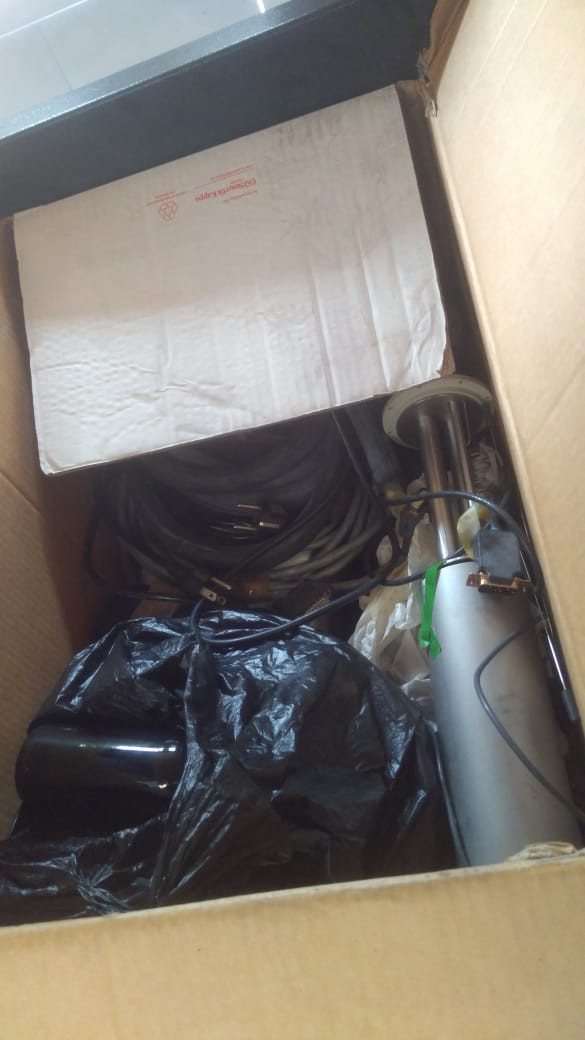
\includegraphics[width=0.24\linewidth]{../Tesis/Figures/process/box1} & 
			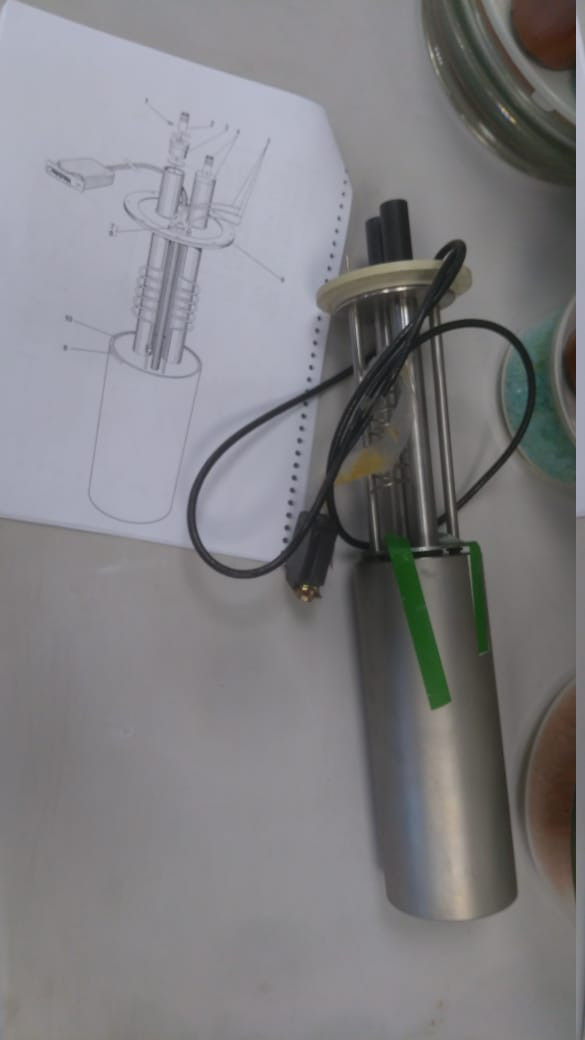
\includegraphics[width=0.24\linewidth]{../Tesis/Figures/process/holder} &
			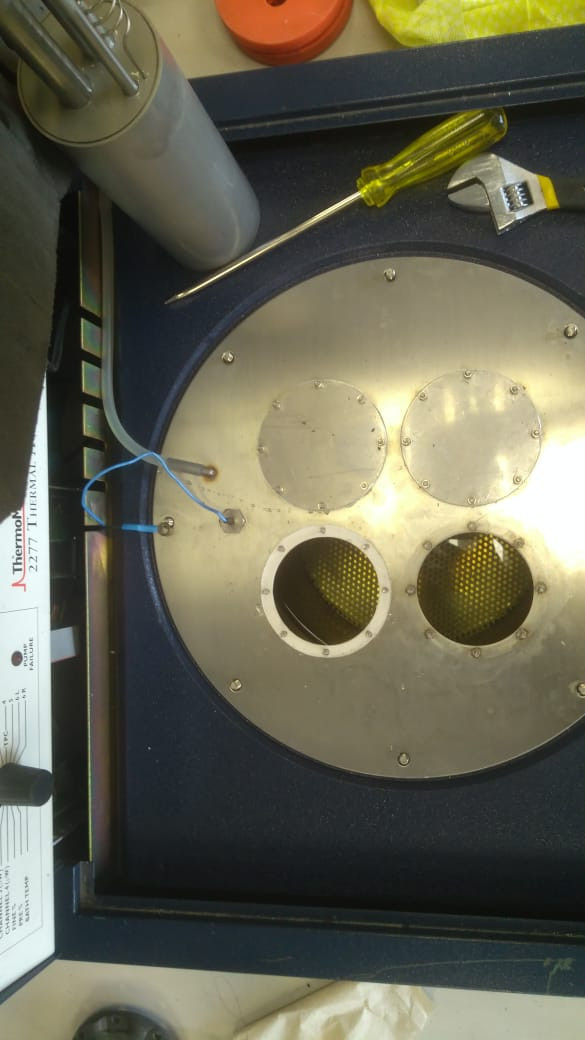
\includegraphics[width=0.24\linewidth]{../Tesis/Figures/process/p1} & 
			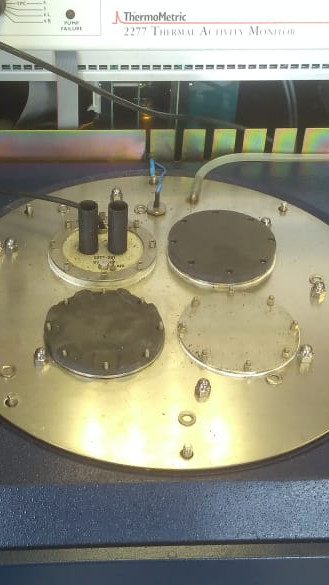
\includegraphics[width=0.24\linewidth]{../Tesis/Figures/process/p2} \\ 
			& 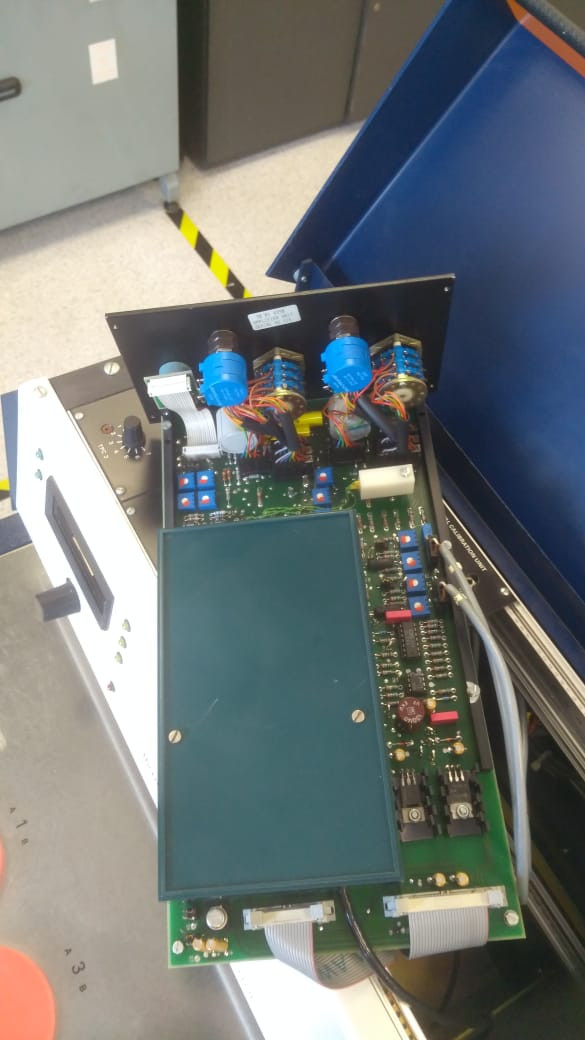
\includegraphics[width=0.24\linewidth]{../Tesis/Figures/process/p3} & 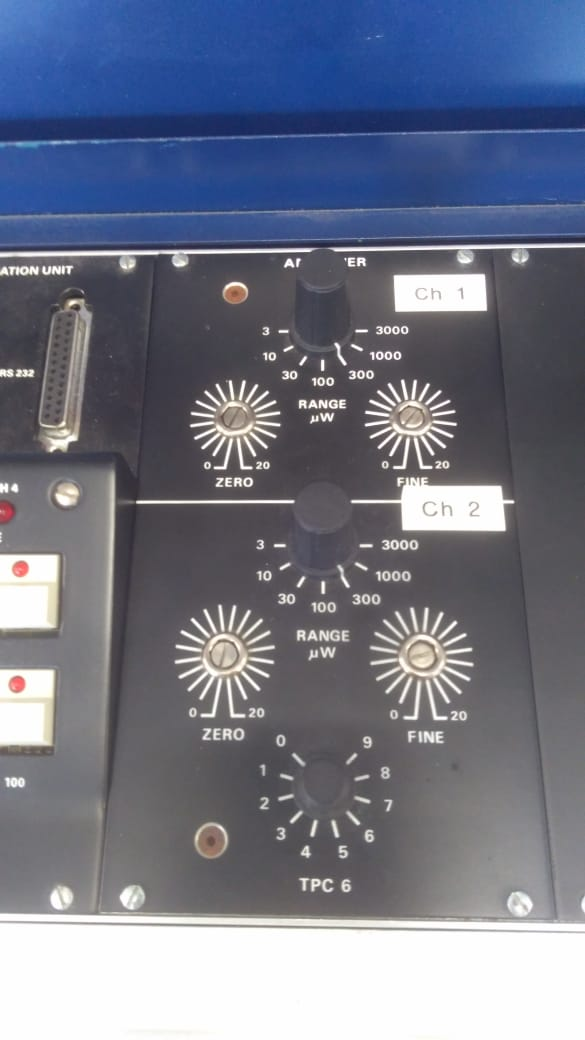
\includegraphics[width=0.24\linewidth]{../Tesis/Figures/process/p4} \\
		\end{tabular}
		\caption{Proceso de instalación de un cilindro de medición.}
	\end{figure}

\section{Instalaci\'on del calor\'imetro}
\section{Control de la temperatura}
\section{Calibraci\'on El\'ectrica}
\section{Calibraci\'on Qu\'imica}
\section{Conclusiones}
\section*{Referencias}
\section*{Agradecimientos}



\end{multicols}
\end{document}